
\chapter{ZÁKLADNÍ INFORMACE O MATEŘSKÝCH ŠKOLÁCH SROVNÁVANÝCH ZEMÍ}
%TODO JA; nejaky kecy tady

	\section{Zařazení mateřské školy v rámci klasifikace vzdělávacího systému}

		V roce 1976 vydalo UNESCO Mezinárodní standardní klasifikaci vzdělávání ISCED (International Standard Classification of Education), která slouží \textit{\uv{jako nástroj vhodný pro shromažďování, zpracování a zpřístupňování vzdělávacích statistik jak v jednotlivých zemích, tak v mezinárodním měřítku"}} \citep{ISCED2}. 

		Klasifikace kmenových oborů vzdělávání z roku 1997 má 7 úrovní vzdělávání (0 až 6).
		Pro účely této práce je důležité si představit první dvě úrovně:

\begin{itemize}
	\setlength\itemsep{-2mm}
	\item [] \textbf{ISCED 0} - Vzdělávání v raném dětství (preprimární vzdělávání,mateřské školy). Programy na této úrovni mají podporovat poznávací, fyzický, sociální a emocionální rozvoj malých dětí, uvádět je do organizované výuky mimo kontext rodiny a rozvíjet jejich emocionální dovednosti nezbytné pro školní docházku a zapojení do společnosti. 
	\item [] \textbf{ISCED 1} - Primární vzdělávání (základní vzdělání, základní školy včetně speciálních - 1.stupeň, zvláštní školy - 1. a 2. stupeň, pomocné školy - nižší, střední a vyšší stupeň a rehabilitační třídy). Programy na této úrovni mají žákům poskytovat základní dovednosti ve psaní, čtení a počítání a vytvářet pevný základ pro učení a porozumění jádru vědění, pro osobní a sociální rozvoj v rámci přípravy na nižší sekundarní vzdělávání. \citep{ISCED}
\end{itemize}

		Preprimární vzdělávání neboli také předškolní vzdělávání spádá do úrovně ISCED 0. Jedná se nepovinné vzdělávání, které uvádí děti raného věku do prostředí institucionálního zařízení. 

		Podle \citet{KeyData} se v mateřských školách v evropských zemích uplatňují různé modely:
		\textit{\begin{enumerate}[1)]
			\setlength\itemsep{-2mm}
			\item \uv{Školský model (school model) – preprimární vzdělávání je organizované ve třídách, v nichž jsou zařazeny děti podle věkových kategorií, tedy podobně jako ve skutečné škole. 
			\item Rodinný model (family model) – preprimární vzdělávání je organizováno ve skupinách sdružujících děti různého věku, tedy podobně jako ve skutečných rodinách. 
			\item Oba modely}
		\end{enumerate}}
		\citep{Prucha99}

		Tyto modely jsou však odlišné i svými vždělávacími cíli. Školský model připravuje děti na vstup do základní školy, kdežto rodinný typ se věnuje spíše rozvoji sociálních dovedností a uvedení dětí do společnosti.

		Realizace předškolního vzdělávání se liší zemi od země. Různé jsou jak cíle tak obsah vzdělávání. Pro porozumění tedy v dalších kapitolách uvádím pozici, kterou mají mateřské školy ve vzdělávacím systému obou sledovaných zemí. 
		

	\section{Mateřské školy ve Francii}
	\label{msvefr}


		\begin{figure} [h!]
			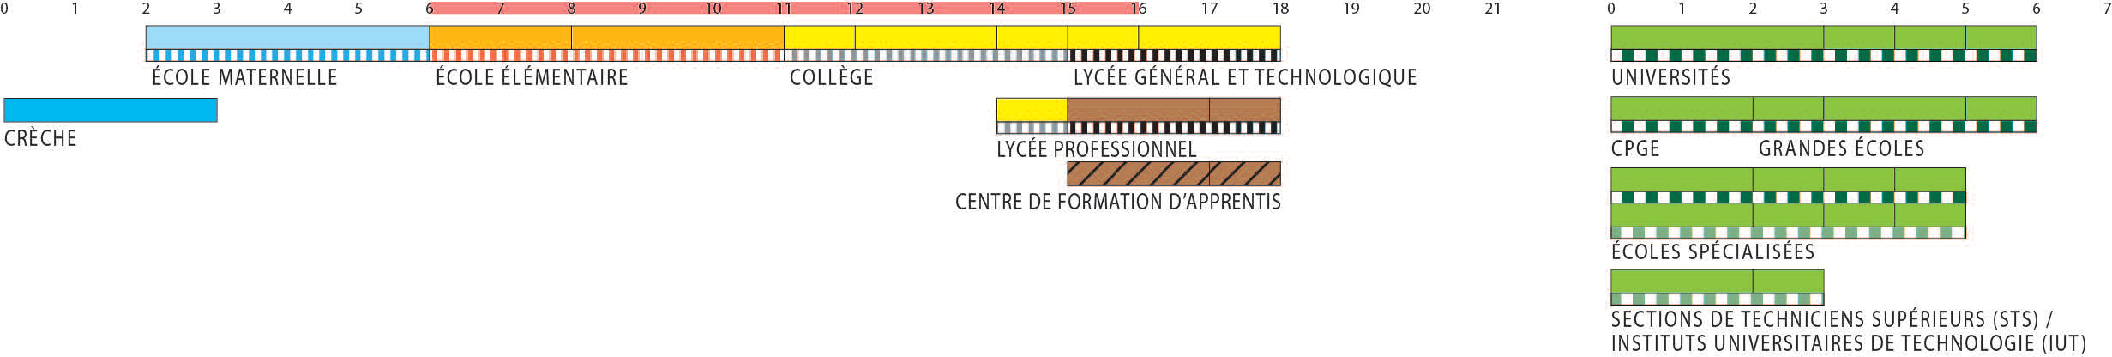
\includegraphics[width=1.0\linewidth]{fotky/msFR.png} \\
			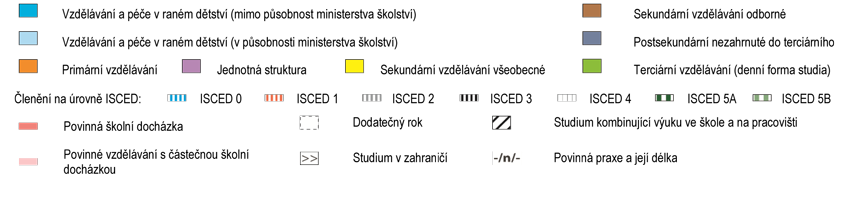
\includegraphics[width=1.0\linewidth]{fotky/msVysvetlivky.png}
			\caption{ \textbf{Materske skoly FR.}
				TODO: 1-2 vety, btw nejsem si jisty jestli to bude citelne...
			}
			\label{obr:msFR}
		\end{figure}
%TODO obrazek
		Mateřské školy ve Francii jsou státní instituce zajišťující preprimární vzdělávání. Dlouholetá tradice nahlíží na předškolní vzdělávání (école maternelle) jako na počáteční formu vzdělávání, na níž navazuje primární vzdělávání (école élémentaire). Jde o návaznost ISCED  úrovně 0 a 1. Mateřská škola poskytuje péči dětem od 2 do 6 let, je však součástí základního vzdělávání poskytující vzdělávání pro děti od 2 do 11 let.

		Primární vzdělávání ve Francii se odehrává ve 3 cyklech. Prvním cyklem (cycle des apprentissages premiers)je mateřská škola, poslední třída mateřské školy (grande section) je již přechodem do druhého cyklu (cysle des apprentisages fondamentaux), jehož součástí je přípravná třída (cours préparatoire CP), na kterou navazují první třída základního vzdělávání (cours élémentaire CE1). Ve třetím cyklu (cycle des approfondissements) je druhá třída základního vzdělávání (cour élémentaire CE2 a dvě střední třídy (Cours moyenne CM1 a CM2). Poté děti přecházejí na sekundární vzdělávání na collège, které odpovídá našemu druhému stupni základních škol. 

		Vzdělání v mateřských školách odpovídá tzv. prvnímu učebnímu cyklu (cycle des apprentissages premiers), rozdělenému do tří stupňů podle věku žáků: nižší stupeň (petite section) pro děti tří až čtyřleté; střední stupeň (moyenne section) pro děti čtyř až pětileté; vyšší stupeň (grande section) pro děti pěti až šestileté.
		(Průcha, 2012). 
% TODO JA: reference prucha
		Je-li v mateřské škole dostatek místa, jsou přijímany děti již od 2 let do tzv. toute petite section. 

\begin{spacing}{1.0}
\begin{table}[h]
	\small
	\begin{center}
	\begin{tabular}{|c|c|c|c|}
		\hline
		\rowcolor{grey}
		\textbf{Cyklus}				& \textbf{Třída}		& \textbf{Věk}	& \textbf{Kde se odehrává}	\\
		\hline
		\hline
		\rowcolor{grey!10}
		%==================================================================================================
		cycle des apprentissages	& toute petite section 	& 2-3 		&				\\ \rowcolor{grey!10}
		premiers (1. cyklus)		& petite section 		& 3-4 		& jen v MŠ 		\\ \rowcolor{grey!10}
									& moyenne section 		& 4-5 		& 				\\ \rowcolor{grey!10}
		\hline
		%==================================================================================================
		cycle des apprentissages 	& grande section 		& 5-6 		& začíná v MŠ, 		\\ \rowcolor{grey!10}
		fondametaux (2.cyklus) 		& CP 					& 6-7 		& pokračuje na ZŠ 	\\ \rowcolor{grey!10}
									& CE1 					& 7-8 		& 					\\ \rowcolor{grey!10}
		\hline
		%================================================================================================+=
		cycle des approfonissements & CE2 					& 8-9 		&					\\ \rowcolor{grey!10}
		(3.cyklus)					& CM1 					& 9-10 		& jen v ZŠ 			\\ \rowcolor{grey!10}
									& CM2 					& 10-11 	& 					\\ \rowcolor{grey!10}
		\hline
	\end{tabular}
	\end{center}
	\caption{ \textbf{Primární vzdělávání ve Francii.} Tabulka znázorňuje věkové rozdělení do tříd a učebních cyklů a barevně je označen přechod mezi mateřskou školou a školou základní. 
	}
	\label{tab:rozdeleniTridCR}
\end{table}
\end{spacing}
		Školství ve Francii je od svých počátků centralizované. Od roku 1982 začala jeho decentralizace, která přerozdělila pravomoc státní administrativy a lokálních samospráv. Stát zůstává garantem vzdělávání jako veřejné služby a definuje rámec vzdělávání a kurikula. Mateřské školy jsou pod pravomocí Ministerstva školství (Ministère de l´éducation national)
%TODO odkaz
%(http://www.clovekvtisni.cz/uploads/file/1360764270-an_KA3_komparace.pdf)

		V roce 1886 byl vydán zákon, podle kterého jsou mateřské školy veřejné, bezplatné a sekulární instituce, a který vymezuje jejich vzdělávací funkce.
%TODO JA principy



	\section{Mateřské školy v České republice}
%TODO obrazek
\begin{figure} [h!]
			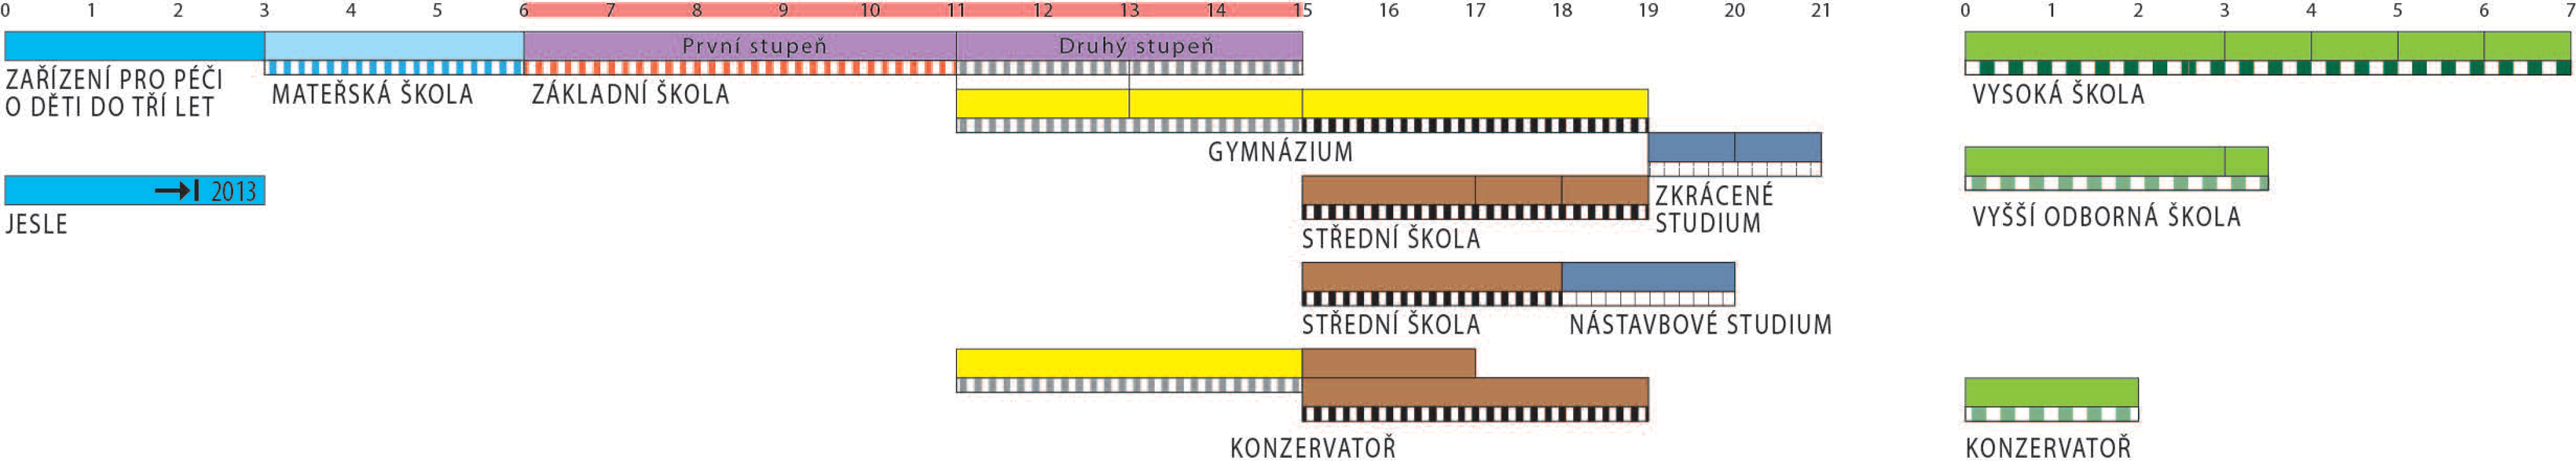
\includegraphics[width=1.0\linewidth]{fotky/msCR.png} \\
			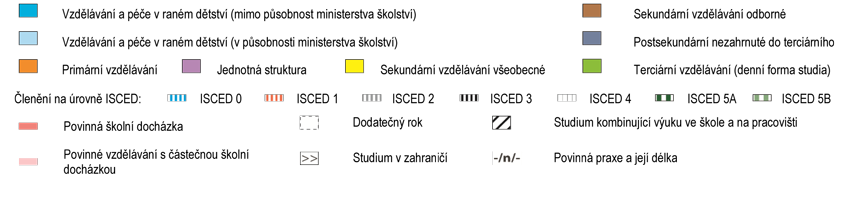
\includegraphics[width=1.0\linewidth]{fotky/msVysvetlivky.png}
			\caption{ \textbf{Materske skoly CR.}
				TODO: 1-2 vety, btw nejsem si jisty jestli to bude citelne...
			}
			\label{obr:msCR}
		\end{figure}

		Mateřská škola v České republice je instituce zajišťující předškolní vzdělávání pro děti od 3 do 6 let (do 7 let v případě odkladu školní docházky), které se školským zákonem stalo legitimní součástí systému vzdělávání. Podle mezinárodní klasifikace se jedná o ISCED 0. Jedná se o organizované vzdělávání, které musí splňovat požadavky MŠMT (Ministerstva školství, mládeže a tělovýchovy). Předškolní vzdělávání v mateřské škole je veřejnou, nepovinnou a bezplatnou službou pro všechny děti. Přednostně jsou přijímány děti v posledním roce před začátkem povinné školní docházky. 

		

		Ve veřejné sféře je zřizovatelem mateřské školy většinou obec nebo svazek obcí. V České republice existují i soukromé mateřské školy.

		Organizačně se mateřská škola dělí na třídy, které je možné vytvářet podle věku, a to na třídy věkově homogenní a na třídy věkově heterogenní. Do mateřských škol je možné zařazovat i děti se specifickými potřebami a vytvářet tak třídy integrované. 

		
		Předškolní vzdělání v mateřské škole má 3 ročníky:
		
	\textit{\begin{itemize}
		\setlength\itemsep{-2mm}
		\item [] \uv{V prvním ročníku mateřské školy se vzdělávají děti, které v příslušném školním roce dovrší nejvýše 4 roky věku.
		\item [] V druhém ročníku mateřské školy se vzdělávají děti, které v příslušném školním roce dovrší nejvýše 5 let věku.
		\item [] Ve třetím ročníku mateřské školy se vzdělávají děti, které v příslušném školním roce dovrší 6 let věku a děti, kterým byl povolen odklad povinné školní docházky.} \citep[s.~71]{Organizace}
	\end{itemize}}

	\begin{spacing}{1.0}


\begin{table}[h]
	\small
	\begin{center}
	\begin{tabular}{|c|c|c|c|}
		\hline
		\rowcolor{grey}
		\textbf{Typ skupiny} & \textbf{Ročník} & \textbf{Věk}	\\
		\hline
		\hline
		\rowcolor{grey!10}
		%==================================================================================================
		homogenní	& 1.ročník 	& 3-4 		\\ \rowcolor{grey!10}
		skupina		& 2.ročník 	& 4-5 		\\ \rowcolor{grey!10}
					& 3.ročník 	& 5-6/7		\\ \rowcolor{grey!10}
		\hline
		%==================================================================================================
		heterogenní & 1.-3.ročník 	& 3-6/7 	\\ \rowcolor{grey!10}
		skupina 	&				&			\\ \rowcolor{grey!10}
		\hline
	\end{tabular}
	\end{center}
	\caption{ \textbf{Rozdělení tříd podle věku v České republice}
	}
	\label{tab:primarniVzdelavaniFR}
\end{table}
\end{spacing}

%TODO JA preformulovat
Přes formální shodu postavení mateřské školy ve vzdělávacím systému obou sledovaných zemí je třeba poukázat na naprosto zásadní rozdíly v cílech mateřských škol a pohledu na dítě, které ji navštěvuje.
Předškolní výchova ve Francii tak jako ve většině románských zemí je charakteristická tím, že naplňuje cíl uvádět dítě do světa školy. Tzn. směřovat práci v mateřské škole k přípravě na vstup do povinné školní docházky. Tento přístup je hluboce tradičně zakořeněn, a tak jak je možné si všimnout při rozboru kurikul, směřuje k získání základních kulturních technik, na nichž je postaven počátek primárního vzdělávání. 

Předškolní vzdělávání v České republice nebylo takto jednoznačně orientované ve své historii, tj. příprav na školu, přeste však tento aspekt vyplynul jako nezbytnost s přijetím dokumentu \uv{Další rozvoj výchovně vzdělávací soustavy} v roce 1976. Tehdy byl cíl mateřských škol zúžen na přípravu pro povinné vzdělávání. Děti, které neabsolvovaly mateřskou školu, byly při zápisech do základní školy vyzvány k náhradnímu opatření, tzn. přípravných tříd, alespoň na dobu 3 měsíců, neboť dovednosti a znalosti získané před nastupem do 1. třídy byly východiskem, na nichž 1. třída \uv{startovata}. Současná mateřská škola není vázána konceptem na školu, její koncept je mnohem širší. Příprava na život v sobě zahrnuje také připravu na povinnou školní docházku. Ovšem v kontextu socializace a radostného dětství s ostatnimi dětmi, tj. \uv{rosteme společně}. Současná předškolní výchova v České republice neni ani školský model, ani rodinný model, ale je to smíšený model obou černobíle postavených typů.

Vzdělávací systemy jsou odlišné, i když by se na první pohled zdálo, že mateřská škola přijímající děti od 2 do 6 let má svou stejnou pozici. Historicky byla francouzská mateřská škola vyjímána vždycky jako vzdělávací instituce. Opravdu tvoří první článěk vzdělávací soustavy (ale nepovinný), o to je překvapivější, že cykly, které dítě v předškolním věku prochází jsou vnímány jako nezbytný obsah na niž se váže povinná školní docházka. Tento stav se jeví jako anomálie. Přestože je nepovinná, 100\% 5ti letých dochází. Všechny rodiny, které žádají o vstup dětí ve 3 letech jsou přijati (ne 2letí).

Tradice české mateřské školy je rovněž velmi dlouhá, ale její pozice jako vzdělávací instituce se vztahuje až ke školskému zákonu, kdy je zařazena jako první článěk vzdělávací sousty. Po roce 1948 se pozice MŠ více blížila sociálnímu zařízení, než skutečně výchovně vzdělávacímu. Mezi lety 1948 a 1989 je její vzdělávací charakter nespochybnitelný. Po roce 1989 byl krátkodobě zpochybněn vzdělávací charakter ve prospech pozice sociální, avšak na konci 90. let, zvláště pak školským zákonem v roce 2004 se její pozice zakotvila a posílila. 
